\section{Every Bureaucrat's  Dilemmas\label{sec:dilemma-trilemma}}

% Not included here: 
% https://en.wikipedia.org/wiki/The_Innovator%27s_Dilemma
% because it is the etic view of change


When a decision has two viable options (neither being best), that presents a \href{https://en.wikipedia.org/wiki/Dilemma}{dilemma}. The name for a decision with three viable options is a \href{https://en.wikipedia.org/wiki/Trilemma}{trilemma}. This section describes a bureaucrat's experience of operating within an organization in terms of dilemmas and trilemmas. Instead of focusing on moral dilemmas (see~\cite{2017_Zacka}) or institutional ethics, here I focus on interpersonal relationships and the logistics of allocating attention. 
% https://en.wikipedia.org/wiki/Defeasible_reasoning

%Dilemma are not unique to bureaucracy. 
Dilemmas are a \href{https://en.wikipedia.org/wiki/Defeasible_reasoning}{simple way} of discussing decisions. % but are not the only relevant aspect of bureaucracy.
Dilemmas are a useful framing to highlight the following concepts:
\begin{itemize}
    \item You, an individual bureaucrat, face decisions that you may not have recognized. Failing to recognize a choice (an error by omission) can lead to suboptimal results. The dilemmas below are generic to any bureaucratic process and are intended to stimulate your ability to identify decisions. 
    \item You face complex trade-offs in your role as a bureaucrat. Dilemmas are intended an entry point to more nuanced reflection that is specific to your situation. The dilemmas below are not exhaustive; this list is merely illustrative. 
    \item You can use dilemmas as an entry to \href{https://en.wikipedia.org/wiki/Theory_of_mind}{intellectual empathy} with fellow bureaucrats when you recognize they face the same dilemmas. These dilemmas are generic to the situation and the person facing the decisions. You now have a topic to discuss with them. You can share your understanding. 
    \item You can be curious about the choice other bureaucrats select for a given dilemma. Everyone in the organization faces these decisions, so these dilemmas give you a topic of conversation to better understand each bureaucrat's view.
    \item You can identify and negotiate potential sources of friction. Other bureaucrats may arrive at different selections for a given dilemma, so recognizing this and discussing it can improve the effectiveness of all involved.
\end{itemize}


% claim
Dilemmas explain the inherent complexity of bureaucracy even when bureaucrats are honest and the purpose of the organization is clear.
% relevance
The point isn't that one should \href{https://en.wikipedia.org/wiki/False_dilemma}{select one of the two options}. The point of recognizing a dilemma is that it is a marker that there is a decision to be made.
% consequence
Once the need for a decision is identified, the action for the bureaucrat is not to select one of the two options. The effective bureaucrat identifies nuances, enumerates alternatives, and talks with fellow bureaucrats about these decisions. Rather than seeking consensus, strive for comprehension of other people's perspective. That way you can navigate decision making processes more effectively.

The choices described below in the simplified representation of dilemmas are intended as a starting point for introducing the decision space relevant to individual bureaucrats. Do not accept the dilemmas presented here as the final framing. Thinking in terms of a limited spectrum of opportunities neglects nuances that enable more creative approaches. 
Awareness of these dilemmas and trilemmas are intended to spark creative imagination about the nuances specific to your situation.

By recognizing the deficiencies of dilemmas, you can identify nuances specific to the situation you are in. Instead of responding to the recognition of a decision with ``should I do this or that?'' the better option is to assess the complexities and \href{https://en.wikipedia.org/wiki/Brainstorming}{brainstorm} multiple options. Talk with stakeholders and understand the history of the situation before making a choice.



\subsection*{How Dilemmas Arise in Bureaucracy}

Given a task, the simplest response for an individual is to take action and be done. There wasn't a decision needed.

If the task is more challenging then first make a plan and then take action and be done. The source of the challenge may be task complexity, scale, number of people impacted, diversity of stakeholders, amount of time needed, how the current task shapes future options, number of collaborators. Regardless of why the task is challenging, a dilemma has already arisen: how much time to spend planning versus doing. 

If the task is even more challenging, it may be useful to gather data for the plan, then make a plan, then take action and be done. A new dilemma arises: how much time to spend gathering data versus planning. The previous dilemma still exists -- how much time to invest in planning versus doing. As an alternative to the dilemma framing, how much time should be allocated to three categories of activity?

But wait, how did the person in the first scenario (just do the task) know no plan was necessary? Either it was an explicit choice or they didn't perceive the need to decide about whether to plan. Someone else faced with that same task might choose differently, e.g., to make a plan. The task complexity is relative to the person's skills, experiences, expectations about stakeholders, and potential ramifications.

In this escalating sequence of increasingly challenging tasks, now suppose the task involves you and another person. The overhead of coordination inflicts additional dilemmas. The examples of complexity arising from coordination are identified in the list of dilemmas below, e.g. \ref{table:micromanaging}, \ref{table:early-intervention}.

An independent source of friction for distributed decision making and distributed knowledge is when people involved in the task don't agree on how challenging it is. The framing of the difficulty matters because it can lead different participants to distinct conclusions about how much time should be spent planning versus for carrying out the action. The choice of ``how complicated is the task?'' shapes the team dynamics and informs the need for hierarchical roles. 

\subsection*{Folk Wisdom on Decision Making}

Bureaucrats, whether hired for their expertise or simply to provide labor, are rarely experts on decision making. There are multiple domains in which \href{https://en.wikipedia.org/wiki/Decision_theory}{decision making} is studied (e.g., \href{https://en.wikipedia.org/wiki/Rational_choice_theory}{economics}, \href{https://en.wikipedia.org/wiki/Game_theory}{mathematics}, \href{https://en.wikipedia.org/wiki/Decision-making}{psychology}), but practicing bureaucrats are more likely familiar with colloquialisms that feel descriptive. A few are provided here to give a sense of both the conciseness and the lack of action embedded in each meme.

\ \\
\href{https://en.wikipedia.org/wiki/Hick\%27s_law}{Hick's law}:
\marginpar{[Tag] Folk Wisdom} 
``Increasing the number of choices will increase the decision time logarithmically.''
\index{folk wisdom!\href{https://en.wikipedia.org/wiki/Hick\%27s_law}{Hick's law}}

\ \\
\href{https://en.wikipedia.org/wiki/Hanlon\%27s_razor}{Hanlon's razor}:
\marginpar{[Tag] Folk Wisdom}
``Never attribute to malice that which is adequately explained by stupidity.''
\index{folk wisdom!\href{https://en.wikipedia.org/wiki/Hanlon\%27s_razor}{Hanlon's razor}}

\ \\
\href{https://en.wikipedia.org/wiki/Parkinson\%27s_law}{Parkinson's law}:
\marginpar{[Tag] Folk Wisdom}
``Work expands so as to fill the time available for its completion.''
\index{folk wisdom!\href{https://en.wikipedia.org/wiki/Parkinson\%27s_law}{Parkinson's law}}

\ \\
\href{https://en.wikipedia.org/wiki/Murphy\%27s_law}{Murphy's law}:
\marginpar{[Tag] Folk Wisdom} ``Anything that can go wrong will go wrong.''
\index{folk wisdom!\href{https://en.wikipedia.org/wiki/Murphy\%27s_law}{Murphy's law}}

\ \\
\href{https://en.wikipedia.org/wiki/Law_of_triviality}{Law of Triviality}:
\marginpar{[Tag] Folk Wisdom}
``People within an organization commonly or typically give disproportionate weight to trivial issues.''
\index{folk wisdom!\href{https://en.wikipedia.org/wiki/Law_of_triviality}{Law of Triviality}}

\ \\

Each of these memes feel descriptive to the practicing bureaucrat. They survive because of their self-encapsulation; no additional thought needed.

In comparison to the folk expressions above, dilemmas are intended to be accessible to practicing bureaucrats and trigger reflection and discussion. Effective action is enabled by improved understanding of the trade-offs faced within an organization. Rather than being reductive, the purpose of cataloging bureaucratic dilemmas is to first point out that there is a choice. Once the choice is recognized, look for ways to think beyond the dichotomy.

\subsection*{How Dilemmas Oversimplify}

Although the following concepts are presented as dilemmas and trilemmas, these are necessarily simplifications. For example, two ways to simplify situations into a dilemma are
\begin{itemize}
    \item Start with a single variable, e.g., ``how much data gathering", and force it into a binary choice ``more data gathering" versus ``less data gathering."
    
    % a reduction of a complicated situation to one variable. 
    \item Start with a complex trade-off space with many opportunities and reduce it to a \href{https://en.wikipedia.org/wiki/False_dilemma}{false dichotomy} of \href{https://en.wikipedia.org/wiki/Zero-sum_thinking}{zero-sum options}: ``more data gathering" vs ``more planning." The actual trade-space involves optimization of multiple goals, like (maximize productivity) and (minimize unnecessary risk) and (maximize quality) and (maximize employee satisfaction) and (minimize latency). 
    % https://bennorthrop.com/Essays/2022/code-ownership-stewardship-or-free-for-all.php
\end{itemize}
The over-simplifications listed below neglect both the continuous nature of the trade-offs and the alternative creative approaches to a specific situation. 

%\subsection*{Dilemmas as a Framing to Ease you into Complexity}



Ponder these dilemmas prior to the pressure of real-time decision making.  Recognize dilemmas and trilemmas and then extend your analysis beyond them by adapting to the local conditions and specific people available to help.
Dilemmas should not be resolved alone. Talk with subordinates,peers, mentors, supervisor.


Once a dilemma is recognized, it is easier to defer and avoid the  decision making process\footnote{\href{https://xkcd.com/1445/}{https://xkcd.com/1445/}\index{xkcd!\href{https://xkcd.com/1445/}{1445}}}. Therefore implementation takes longer necessary. 
This delay is then ripples down the chain of dependencies. 

\subsection*{Dilemmas are not Purely Intellectual}
Decision making is not a purely intellectual task; there is emotional stress induced by the process. Dilemmas create cognitive dissonance for the decision maker. Any selection is going to have downsides, and any compromise will be suboptimal. Those burdens weigh morally on deciders because of the consequences on other people.

To counter this morale weight, talk with other people about decisions. 
\marginpar{[Tag] Actionable Advice}
Even if this does not alleviate the responsibility of deciding, discussion can help you arrive at new insights. 

\subsection*{More Complications}
Adding to the difficulty and stress, dilemmas presented here occur concurrently and continuously. The dilemmas are inter-dependent due to both to the common variables and the constrained resources.
Selecting an option for one dilemma alters the options available in other dilemmas.

Oscillation between approaches can be caused by change of management, accumulation of experience (dissatisfaction) with one solution, the desire for promotion within the hierarchy (where change is presented as progress), or a desire for cost savings (efficiency). The rate of oscillation is an indicator of the half-life of \href{https://en.wikipedia.org/wiki/Institutional_memory}{institutional memory for an organization}.  

The dilemmas identified below for generic bureaucracy are just a baseline. For the culture you are in and the project you're working on and the people you're working with, there will be additional dilemmas to identify. 

\ \\

The following two sections categorize dilemmas as \hyperref[sec:personal-policy-dilemmas]{personal policies} 
%\iftoggle{sectionref}
and policies regarding \hyperref[sec:org-dilemma]{structure of the organization}.
%\iftoggle{sectionref}
The personal policies apply to each bureaucrat in an organization, while the structural policies for an organization are faced by a subset of bureaucrats in the management role. 

\subsection*{Personal Policy Dilemmas \label{sec:personal-policy-dilemmas}}

In practice, the following decisions are unordered and are constantly faced by the bureaucrat. As observed by Lindblom in~\cite{1959_Lindblom}, this flurry of decisions contrasts to a regularized process that might be envisioned as optimal.


% https://graphthinking.blogspot.com/2019/08/two-misleading-simplifications-when.html
\begin{center}
\begin{table}[H] % ht
\begin{tabular}{ | m{\dilemmatablewidth}| m{\dilemmatablewidth} | } 
  \hline
  \textbf{Focus on the immediate problem.} &
  \textbf{Ponder the systemic issues and adjacent contexts.} \\
  \hline
  \textit{Description}: Focus on isolated problematic aspects and do worry about the interdependencies and feedback loops and stakeholder incentives. &
  \textit{Description}: Philosophical musings with a holistic view. \\
  \hline
  \textit{Cons}: Misses systemic issues, causes that exist outside the immediate scope, or issues that occur due to interacting processes. & 
  \textit{Cons}: Relies on knowledge of the wider system that you may have less awareness of. Less emphasis on getting things done. May reveal problems that you don't have authority to address. \\
  \hline
\end{tabular}
\caption{
\textit{Dilemma of Aperture.}
\index{dilemma!of aperture}
Scope of problem solving can be narrow or broad. Rather than limit your investigations to one or the other, flipping between the two on a recurring basis (but not too often) can help.
}
\label{table:focus-vs-systemic}
\end{table}
\end{center}

The \href{table:focus-vs-systemic}{Dilemma of Aperture} is defined in terms of scope. An adjacent dilemma is the question of duration of tasks: short-term or long-term. The right balance of how long tasks take is more project management then bureaucratic. I try to identify a small number of long-term tasks, then divide each into smaller (shorter) tasks. The dependencies of the smaller tasks then determine the order of the work.

% How does this relate directly to bureaucracy as defined as shared resource management policymaking?
The \href{table:focus-vs-systemic}{Dilemma of Aperture} is not specific to bureaucracy, but commonly arises because isolated problems rarely exist. Challenges occur as part of larger systemic contexts. Addressing the immediate problem leaves the system issue, and tackling system issues are more difficult. 

% How does this impact your relationships with other bureaucrats?
Your selection of narrow versus wide within the \href{table:focus-vs-systemic}{Dilemma of Aperture} depends on what you find emotionally rewarding. Other bureaucrats may gain emotional enjoyment from approaches to problem solving that you do not. Finding ways to leverage that difference (rather than minimizing it) is useful. 

% Are the incentive structures aligned to support one direction or the other?
Organizations typically incentivize short-term behavior. Annual performance reviews and quarterly feedback cycles might miss systemic changes that take multiple years to enact. Identifying incremental milestones is one response, though that isn't always feasible. Another approach is to only report a subset of your activities (the ones that yield short-term results). 

\begin{center}
\begin{table}[H] % ht
\begin{tabular}{ | m{\dilemmatablewidth}| m{\dilemmatablewidth} | } 
  \hline
  \textbf{Speak out/speak up if something is wrong or \href{https://en.wikipedia.org/wiki/Moral_injury}{offends you}.} &
  \textbf{Hold back comments and questions to minimize disruptions.} \\
  \hline
  \textit{Cons}: You could be missing context; you might look stupid. & 
  \textit{Cons}: You missed an opportunity to correct something; you missed an opportunity to get educated about a situation. \\
  \hline
\end{tabular}
\caption{
\textit{Dilemma of Speaking.}
\index{dilemma!of speaking}
There is conflicting folk wisdom on both sides of this dilemma: 
``\href{https://en.wikipedia.org/wiki/The_squeaky_wheel_gets_the_grease}{The squeaky wheel gets the grease}" 
\index{folk wisdom!Squeaky wheel gets the grease}
%\marginpar{[Tag] Folk Wisdom}
and 
``The squeaky wheel gets replaced." 
%\marginpar{[Tag] Folk Wisdom}
\index{folk wisdom!Squeaky wheel gets replaced}
How you raise the issue, with whom, and in what context all matter to either correcting the situation or getting better educated.
}
\label{table:speak-up-or-hold-back}
\end{table}
\end{center}

% How does this relate directly to bureaucracy as defined as shared resource management policymaking?
The \href{table:speak-up-or-hold-back}{Dilemma of Speaking} arises in bureaucracy because different people have different opinions about subjective policy. You may see someone doing something that appears wasteful, but that may be because you're not aware of what the optimization objective is. Or that person may be unaware of the waste, or they may not be aware there is a more effective way to carry out the action. 

Resolving differences of opinion is not always necessary. If all members of and organization were to try to minimize policy distinctions, the members could spend all of their time doing so. 

% How does this impact your relationships with other bureaucrats?
The \href{table:speak-up-or-hold-back}{Dilemma of Speaking} is eased when you have relationships with other bureaucrats that allow you to express your curiosity or uncertainty in a way that doesn't make the person you are talking to feel threatened, or that they are wasting their time explaining what seems obvious. 

% Are the incentive structures aligned to support one direction or the other?
Whether the culture of an organization promotes speaking up or not depends on having either top-down encouragement or relationships that exist outside formal hierarchical roles. 
% TODO: not sure the above statement is valid; need to expand.
  
\begin{center}
\begin{table}[H] % ht
\begin{tabular}{ | m{\dilemmatablewidth}| m{\dilemmatablewidth} | } 
  \hline
  \textbf{Intervene before the deployment of a policy or process or product} &
  \textbf{Wait with feedback until deployment.} \\
  \hline
  \textit{Description}: You may lack relevant context. You may know something the team does not. & 
  \textit{Description}: Allow the team to learn. Allow the team to complete their vision. \\
  \hline
  \textit{Cons}: Engaging prematurely betrays your awareness; future explorations by that team are made less visible. & 
  \textit{Cons}: The team wasted time and attention on something that wouldn't work or may even be harmful. \\
  \hline
\end{tabular}
\caption{
\textit{Dilemma of Early Intervention.}
\index{dilemma!of early intervention}
As an outsider to a team responsible for a process/policy/product, suppose you learn of something prior to official deployment (e.g., you learn the internal musings of another team). There is folk wisdom on both sides: 
``Stay in your own lane'' 
\index{folk wisdom!Stay in your own lane}
%\marginpar{[Tag] Folk Wisdom}
and 
``Speak up when you see something wrong.''
\index{folk wisdom!Speak up when you see something wrong}
%\marginpar{[Tag] Folk Wisdom}
See the related \href{table:micromanaging}{Dilemma of Micromanaging} in Table~\ref{table:micromanaging}.}
\label{table:early-intervention}
\end{table}
\end{center}

% How does this relate directly to bureaucracy as defined as shared resource management policymaking?
When there is an objective measure for success, suggestions can be evaluated with respect to whether change improves the outcome. Because bureaucracy is based on subjective policy, there are always differences about how to improve. The \href{table:early-intervention}{Dilemma of Early Intervention} is about knowledge your role didn't require. That knowledge may be incomplete or you may know more than the people taking action. 


% How does this impact your relationships with other bureaucrats?
The \href{table:early-intervention}{Dilemma of Early Intervention} can harm your relationships if you are seen as exceeding your role. Your action can benefit the organization, and the team taking the action may be grateful for the intervention. 

% Are the incentive structures aligned to support one direction or the other?
Because organizations promote individuals, and there are a limited number of promotions available, the naive expectation is that intervention that could benefit others and risks harming your relationships would not happen. The motive for an individual to intervene is the displeasure of watching other people waste time and resources, or the possibility to learn something new.


\begin{center}
\begin{table}[H] % ht
\begin{tabular}{ | m{\dilemmatablewidth}| m{\dilemmatablewidth} | } 
  \hline
  \textbf{Review the status of progress for other people early and often. Many milestones, check-ins, and updates.} &
  \textbf{Review status of progress infrequently; just do the work.} \\
  \hline
  \textit{Description}: \href{https://en.wikipedia.org/wiki/Micromanagement}{Micromanagement}. & 
  \textit{Description}: Hands-off management style. \\
  \hline
  \textit{Pros}: Early intervention when things are not going well. & 
  \textit{Pros}: Enables independence. \\
  \hline
  \textit{Cons}: Takes up your time and the people you're reviewing. Conveys low trust. & 
  \textit{Cons}: Team members are unsure how to proceed and don't know what the goal is. \\
  \hline
\end{tabular}
\caption{\textit{Micromanagement from the supervisor's view.}
\index{dilemma!of micromanagement}
An expression of concern and control -- wanting the right outcome, wanting to provide guidance and feedback. Applies to both peers and subordinates.}
\label{table:micromanaging}
\end{table}
\end{center}

% How does this relate directly to bureaucracy as defined as shared resource management policymaking?
\href{table:micromanaging}{Micromanagement from the supervisor's view} is not unique to bureaucratic organizations. The tendency to micromanage does not depend on the level of technical expertise of the manager. Micromanagement occurs when the manager feels insecure about results. If the employees are untrained or unmotivated, the sense of insecurity may be reasonable.

% How does this impact your relationships with other bureaucrats?
Limiting \href{table:micromanaging}{micromanagement from the supervisor's view} means finding an acceptable level of engagement. This depends on the training and motivation of each participant. 

% Are the incentive structures aligned to support one direction or the other?
The manager is accountable for the outcome of the people being supervised, which leads to fear that underlings will fail. 

\begin{center}
\begin{table}[H] % ht
\begin{tabular}{ | m{\dilemmatablewidth}| m{\dilemmatablewidth} | } 
  \hline
  \textbf{Bureaucrat expects management to provide solutions -- just tell members what to do.} & 
  \textbf{Bureaucrat dislikes managers micromanaging by telling people what to do.} \\ 
  \hline
  \textit{Cons}: Your manager may not have insight on what needs to be done. Or they may guide you in a less effective direction. &
  \textit{Cons}: No autonomy, unable to exploit your expertise and creativity. \\  
  \hline
\end{tabular}
\caption{\textit{Micromanagement from the subordinate's view.}
\index{dilemma!of micromanagement for subordinates}
This is the opposite perspective of \ref{table:micromanaging}. Nominally the manager helps identify the goals and provides context and the subordinate figures out how to accomplish the goal, but who is responsible for what is negotiable in each relationship.
}
\label{table:solution_provider}
\end{table}
\end{center}

% How does this relate directly to bureaucracy as defined as shared resource management policymaking?
The \href{table:solution_provider}{Micromanagement from the subordinate's view}
% How does this impact your relationships with other bureaucrats?
The \href{table:solution_provider}{Micromanagement from the subordinate's view}
% Are the incentive structures aligned to support one direction or the other?
  

\begin{center}
\begin{table}[H] % ht
\begin{tabular}{ | m{\dilemmatablewidth}| m{\dilemmatablewidth} | } 
  \hline
  \textbf{Write everything down to \href{https://en.wikipedia.org/wiki/Cover_your_ass}{cover your ass}.} &
  \textbf{Don't record sensitive conversations that could be used against you or others.} \\
  \hline
  \textit{Cons}: Takes a lot of time and effort to accurately capture intent. Recording can be done poorly or be misconstrued.  & 
  \textit{Cons}: No written record to point to when someone changes their behavior. \\
  \hline
\end{tabular}
\caption{\textit{Dilemma of Documentation.}
\index{dilemma!of documentation}
\index{dilemma!of documentation}
I personally write things down and share them with other people (e.g., this book), but there are costs and risks to investing in documentation. There are \href{https://en.wikipedia.org/wiki/Dark_pattern}{dark patterns} for this trade-off, like intentionally misquoting another person to bias the documentation in your favor, or only writing down the aspects of conversation that favor the outcome you are interested in.}
\label{table:notes_or_no_notes}
\end{table}
\end{center}

% How does this relate directly to bureaucracy as defined as shared resource management policymaking?
The \href{table:notes_or_no_notes}{Dilemma of Documentation}
% How does this impact your relationships with other bureaucrats?
The \href{table:notes_or_no_notes}{Dilemma of Documentation}
% Are the incentive structures aligned to support one direction or the other?
  

\begin{center}
\begin{table}[H] % ht
\begin{tabular}{ | m{\dilemmatablewidth}| m{\dilemmatablewidth} | } 
  \hline
  \textbf{Ponder what should or could be done.} &
  \textbf{Figure out how to carry out the goal.}\\
  \hline
  \textit{Description}: Which of these should I select? & 
  \textit{Description}: How should I do the thing I selected? \\
  \hline
  \textit{Cons}: Less time for action. & 
  \textit{Cons}: Prematurely select an action that is suboptimal. \\
  \hline
\end{tabular}
\caption{\textit{Dilemma of Think or Do.}
\index{dilemma!of think or do}
Brainstorming is useful, as is considering the holistic situation. At some point that transitions to action, but when? This is a question of how much time to spend admiring the forest versus the trees. Both of these options an succumb to \href{https://en.wikipedia.org/wiki/Analysis_paralysis}{analysis paralysis}
}
\label{table:forest-vs-trees}
\end{table}
\end{center}

% How does this relate directly to bureaucracy as defined as shared resource management policymaking?
The \href{table:forest-vs-trees}{Dilemma of Think or Do}
% How does this impact your relationships with other bureaucrats?
The \href{table:forest-vs-trees}{Dilemma of Think or Do}
% Are the incentive structures aligned to support one direction or the other?
  

\begin{center}
\begin{table}[H] % ht
\begin{tabular}{ | m{\dilemmatablewidth}| m{\dilemmatablewidth} | } 
  \hline
  \textbf{Allocate time for meetings to facilitate coordination.} &
  \textbf{Allocate time for action.} \\
  \hline
  \textit{Cons}: Less time for participants to implement ideas. & 
  \textit{Cons}: Results in uncoordinated activity which can be wasteful. \\
  \hline
\end{tabular}
\caption{\textit{Dilemma of Coordinate or Do.}
\index{dilemma!of coordinate or do}
Like Dilemma~\ref{table:forest-vs-trees}, but here the question is about coordination versus doing the work. The amount of coordination depends on how many stakeholders there are, how familiar the stakeholders are with the challenge, and whether the action is reversible when found to be incorrect.
}
\label{table:meetings-versus-work}
\end{table}
\end{center}


% How does this relate directly to bureaucracy as defined as shared resource management policymaking?
The \href{table:meetings-versus-work}{Dilemma of Coordinate or Do}
% How does this impact your relationships with other bureaucrats?
The \href{table:meetings-versus-work}{Dilemma of Coordinate or Do}
% Are the incentive structures aligned to support one direction or the other?


\begin{center}
\begin{table}[H] % ht
\begin{tabular}{ | m{\dilemmatablewidth}| m{\dilemmatablewidth} | } 
  \hline
  \textbf{Operate at the level you are being paid for.} &
  \textbf{Operate above the level that you are being paid for in order to be a promoted.} \\
  \hline
  \textit{Description}: Meet job requirements but nothing extra. &
  \textit{Description}: Exceed job requirements. \\
  \hline
  \textit{Cons}: Risk not being promoted. & 
  \textit{Cons}: Experience wage loss since the organization is getting free labor. \\
  \hline
\end{tabular}
\caption{\textit{Dilemma of Working extra hard.}
\index{dilemma!of working extra hard}
Work above your pay grade (provide the organization extra labor and you get reduced pay) or at your pay grade (expected labor and pay)?
}
\label{table:work_extra_or_work_as_expected}
\end{table}
\end{center}

% How does this relate directly to bureaucracy as defined as shared resource management policymaking?
The \href{table:work_extra_or_work_as_expected}{Dilemma of Working extra hard}
% How does this impact your relationships with other bureaucrats?
The \href{table:work_extra_or_work_as_expected}{Dilemma of Working extra hard}
% Are the incentive structures aligned to support one direction or the other?


\begin{center}
\begin{table}[H] % ht
\begin{tabular}{ | m{\dilemmatablewidth}| m{\dilemmatablewidth} | } 
  \hline
  \textbf{Send bad news up the chain of command.} &
  \textbf{Minimize bad news up the chain of command.} \\
  \hline
  \textit{Pros}: You are a reliable source of news. &
  \textit{Pros}: You minimize the burden of managers. \\
  \hline
  \textit{Cons}: You are viewed as a source of problems. & 
  \textit{Cons}: Harmful events eventually catch up with the organization.  \\
  \hline
\end{tabular}
\caption{\textit{Dilemma of Bad News.}
\index{dilemma!of bad news}
The canonical example is the \href{https://en.wikipedia.org/wiki/Space_Shuttle_Challenger_disaster}{Challenger disaster}.}
\label{table:bad-news-up-the-chain}
\end{table}
\end{center}

% How does this relate directly to bureaucracy as defined as shared resource management policymaking?
The \href{table:bad-news-up-the-chain}{Dilemma of Bad News}
% How does this impact your relationships with other bureaucrats?
The \href{table:bad-news-up-the-chain}{Dilemma of Bad News}
% Are the incentive structures aligned to support one direction or the other?


\begin{center}
\begin{table}[H] % ht
\begin{tabular}{ | m{\dilemmatablewidth}| m{\dilemmatablewidth} | } 
  \hline
  \textbf{Prepare for disasters and emergencies, invest in mitigation.} &
  \textbf{Wait for the specific problem to arise before responding.} \\
  \hline
  \textit{Pros}: Lessen the impact when bad things happen; decrease the number of problems from occurring in the first place. &
  \textit{Pros}: Deal with the specifics of the scenario at that time and thus be better informed. Look like a hero for handling emergency. \\
  \hline
  \textit{Cons}: Fewer events evolve into emergencies because you're prepared, or the impact of disasters is lessened. Both make you look overly paranoid and wasteful. Less recognition for planning. & 
  \textit{Cons}: Unexpected events result in worse outcomes.  \\
  \hline
\end{tabular}
\caption{
\textit{Dilemma of Preparation versus Cleanup.} 
\index{dilemma!of preparation and cleanup}
How much to invest in contingency planning and preparedness. In practice you will do both.}
\label{table:emergencies-vs-ignore}
\end{table}
\end{center}

% How does this relate directly to bureaucracy as defined as shared resource management policymaking?
The \href{table:emergencies-vs-ignore}{Dilemma of Preparation versus Cleanup}
% How does this impact your relationships with other bureaucrats?
The \href{table:emergencies-vs-ignore}{Dilemma of Preparation versus Cleanup}
% Are the incentive structures aligned to support one direction or the other?


\begin{center}
\begin{table}[H] % ht
\begin{tabular}{ | m{\dilemmatablewidth}| m{\dilemmatablewidth} | } 
  \hline
  \textbf{Only let good ideas through as determined by a detailed review process of clearly specified plan.} &
  \textbf{Give resources to untested ideas.} \\
  \hline
  \textit{Pros}: Less waste of resources and time. Everyone has confidence in the investment. & 
  \textit{Pros}: High-risk/high-reward ideas that are disruptive can be implemented. \\
  \hline
  \textit{Cons}: Burdensome review process. & 
  \textit{Cons}: some ideas will fail. \\
  \hline
\end{tabular}
\caption{
\textit{Dilemma of Idea filtering.}
\index{dilemma!of idea filtering}
How much vetting should novel ideas get before implementation?
}
\label{table:idea-filtering}
\end{table}
\end{center}

% How does this relate directly to bureaucracy as defined as shared resource management policymaking?
The \href{table:idea-filtering}{Dilemma of Idea filtering}
% How does this impact your relationships with other bureaucrats?
The \href{table:idea-filtering}{Dilemma of Idea filtering}
% Are the incentive structures aligned to support one direction or the other?


% https://graphthinking.blogspot.com/2016/05/claim-innovation-is-either-disruptive.html
\begin{center}
\begin{table}[H] % ht
\begin{tabular}{ | m{\dilemmatablewidth}| m{\dilemmatablewidth} | } 
  \hline
  \textbf{Work on disruptive innovation.} &
  \textbf{Work on iterative (evolutionary) innovation.} \\
  \hline
  \textit{Description}: Start from scratch, aim for revolution, replace the legacy.  &
  \textit{Description}: Starts with change to existing solution, adjust the legacy path.  \\  
  \hline
  \textit{Pros}: High reward. & 
  \textit{Pros}: Low risk, low cost. \\
  \hline
  \textit{Cons}: High risk, high cost. & 
  \textit{Cons}: Low reward. \\
  \hline
\end{tabular}
\caption{\textit{Dilemma of Innovation.}
\index{dilemma!of innovation}
Incremental change may not suffice. Disruption can be costly.
}
\label{table:disruptive-or-iterative}
\end{table}
\end{center}

% How does this relate directly to bureaucracy as defined as shared resource management policymaking?
The \href{table:disruptive-or-iterative}{Dilemma of Innovation}
% How does this impact your relationships with other bureaucrats?
The \href{table:disruptive-or-iterative}{Dilemma of Innovation}
% Are the incentive structures aligned to support one direction or the other?


\begin{center}
\begin{table}[H] % ht
\begin{tabular}{ | m{\dilemmatablewidth}| m{\dilemmatablewidth} | } 
  \hline
  \textbf{Innovate in a novel-to-your-team environment.} &
  \textbf{Innovate in your team's standard environment.} \\
  \hline
  \textit{Pros}: More likely to allows people to drop their expectations.  & 
  \textit{Pros}: Easy to operate in. \\
  \hline
  \textit{Cons}: Loses access to connections vital to actually create success. Use extra space, logistics of moving. & 
  \textit{Cons}: Allows conventional processes to take effect. People hold onto their assumptions. \\
  \hline
\end{tabular}
\caption{
\textit{Dilemma of Where to Innovate.}
\index{dilemma!of where to innovate}
Where (physically, spatially) innovation takes place matters because the environment sets context for assumptions.
}
\label{table:where-to-innovate}
\end{table}
\end{center}

% How does this relate directly to bureaucracy as defined as shared resource management policymaking?
The \href{table:where-to-innovate}{Dilemma of Where to Innovate}
% How does this impact your relationships with other bureaucrats?
The \href{table:where-to-innovate}{Dilemma of Where to Innovate}
% Are the incentive structures aligned to support one direction or the other?


% https://graphthinking.blogspot.com/2016/06/innovation-in-open-versus-behind-curtain.html
\begin{center}
\begin{table}[H] % ht
\begin{tabular}{ | m{\dilemmatablewidth}| m{\dilemmatablewidth} | } 
  \hline
  \textbf{Work on innovation in the open.} &
  \textbf{Work on innovation in hiding.} \\
  \hline
  \textit{Pros}: More likely to be criticized. Criticism can be positive (as in an incubator setting).& 
  \textit{Pros}: Less drama -- the incumbent won't attack the innovation since they don't know about it. \\
  \hline
  \textit{Cons}: Negative criticism intended to harm -- an incumbent has reason to be defensive. The incumbent attacks the innovation before it is sufficiently developed or has time to build a user base. & 
  \textit{Cons}: Less opportunity for feedback. Project is easier to kill since the value is not advertised.\\
  \hline
\end{tabular}
\caption{
\textit{Dilemma of Obfuscated Innovation.}
\index{dilemma!of obfuscated innovation}
How is innovation carried out within the organization?
}
\label{table:innovate-open-obscure}
\end{table}
\end{center}

% How does this relate directly to bureaucracy as defined as shared resource management policymaking?
The \href{table:innovate-open-obscure}{Dilemma of Obfuscated Innovation}
% How does this impact your relationships with other bureaucrats?
The \href{table:innovate-open-obscure}{Dilemma of Obfuscated Innovation}
% Are the incentive structures aligned to support one direction or the other?


\begin{center}
\begin{table}[H] % ht
\begin{tabular}{ | m{\dilemmatablewidth}| m{\dilemmatablewidth} | } 
  \hline
  \textbf{Seek recognition for your work.} &
  \textbf{Work in obscurity.} \\
  \hline
  \textit{Pros}: Helps with promotion. & 
  \textit{Pros}: Less distraction. \\
  \hline
  \textit{Cons}: Devalues the contributions of other people. & 
  \textit{Cons}: No one knows the value of your work and you won't get feedback. \\
  \hline
\end{tabular}
\caption{
\textit{Dilemma of Recognition.}
\index{dilemma!of recognition}
This dilemma is magnified when the task you work on is high risk or is resource intensive. 
}
\label{table:recognition-obscurity}
\end{table}
\end{center}

% How does this relate directly to bureaucracy as defined as shared resource management policymaking?
The \href{table:recognition-obscurity}{Dilemma of Recognition}
% How does this impact your relationships with other bureaucrats?
The \href{table:recognition-obscurity}{Dilemma of Recognition}
% Are the incentive structures aligned to support one direction or the other?


\begin{center}
\begin{table}[H] % ht
\begin{tabular}{ | m{\dilemmatablewidth}| m{\dilemmatablewidth} | } 
  \hline
  \textbf{Gather lots of data.} &
  \textbf{Gather minimal data.} \\
  \hline
  \textit{Description}: Gather lots of data for a well-informed decision. &
  \textit{Description}: Minimal information because decision maker knows what to do or outcome is irrelevant.  \\  
  \hline
  \textit{Cons}: High cost of gathering data (time, resources). \href{https://en.wikipedia.org/wiki/Opportunity_cost}{Opportunity costs}. & 
  \textit{Cons}: Lack of data results in decisions based on oversimplified assessment. \\
  \hline
\end{tabular}
\caption{
\textit{Dilemma of Data Quantity.}
\index{dilemma!of data quantity}
How much data to gather for a decision. See figure~\ref{fig:data_collection_cost_uncertainty}. See also the description of 
 \hyperref[sec:bureaucratic-debt]{bureaucratic debt}.
%\ifsectionref
%in section~\ref{sec:bureaucratic-debt}.
%\fi
%\iftoggle{sectionref}{%
%in section~\ref{sec:bureaucratic-debt}.
%}
%{\tiny Tag: Decision making.}
}
\label{table:gather_data_lots-vs-little}
\end{table}
\end{center}

\begin{figure}[H] % ht
        \centering
        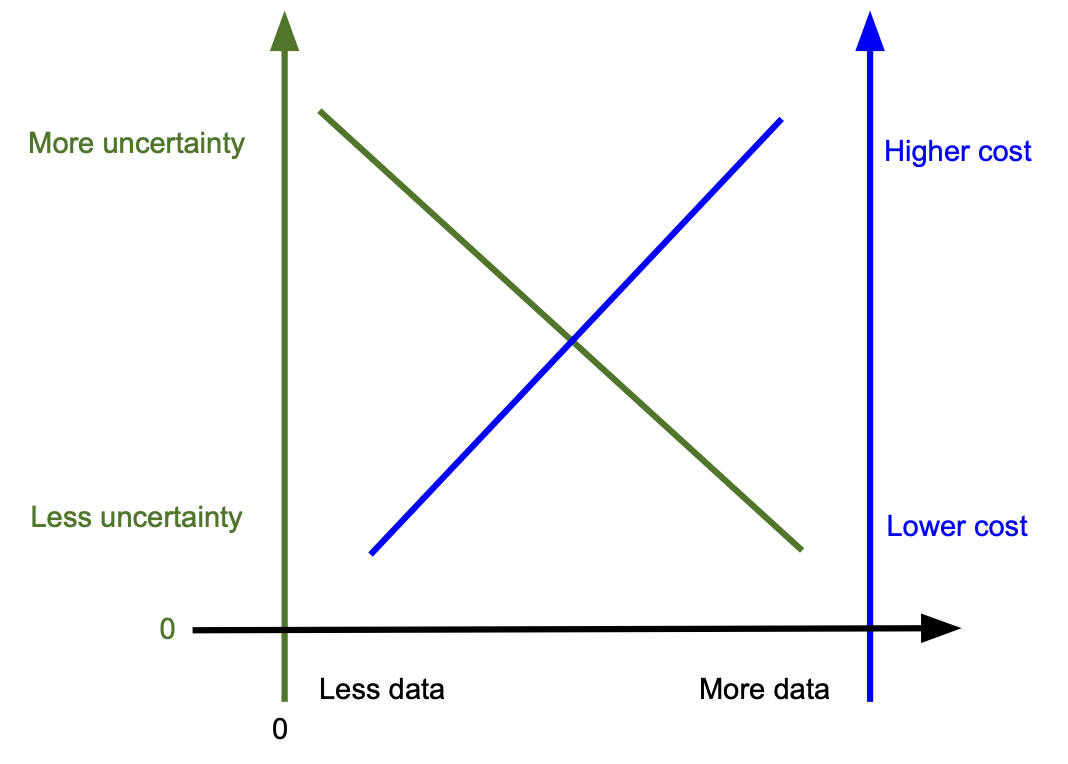
\includegraphics[width=0.8\textwidth]{images/cost_and_uncertainty_for_data_collection}
        \caption{Collecting more data costs money and decrease uncertainty. See Dilemma~\ref{table:gather_data_lots-vs-little}.}
        \label{fig:data_collection_cost_uncertainty}
\end{figure}

The logistics of gathering data can be measured, but there are other subjective aspects to account for as well. Making a decision has an emotional toll on the decider due to the risk of failure. Also, decisions are made in a social context, with decision makers accounting for the ramifications on people they have relationships with. 

% How does this relate directly to bureaucracy as defined as shared resource management policymaking?
The \href{table:gather_data_lots-vs-little}{Dilemma of Data Quantity}
% How does this impact your relationships with other bureaucrats?
The \href{table:gather_data_lots-vs-little}{Dilemma of Data Quantity}
% Are the incentive structures aligned to support one direction or the other?


Gathering data (Dilemma~\ref{table:gather_data_lots-vs-little}) is distinct from planning (Dilemma~\ref{table:planning}). It is possible to do a lot of planning with only a little information gathered, and it is feasible to have lots of data and do no planning. 

\begin{center}
\begin{table}[H] % ht
\begin{tabular}{ | m{\dilemmatablewidth}| m{\dilemmatablewidth} | } 
  \hline
  \textbf{Extensive planning upfront (proactive)} & 
  \textbf{Iterative improvement of plans (reactive)} \\ 
  \hline
  \textit{Description}: Lots of time spent brainstorming potential scenarios and contingency options prior to taking action. & 
  \textit{Description}: Start taking action and use feedback to shape next actions. \\ 
  \hline
  \textit{Cons}: ``No plan survives contact with the enemy.''\footnote{Modified from the original version written by \href{https://en.wikipedia.org/wiki/Helmuth_von_Moltke_the_Elder}{von Moltke}.} & 
  \textit{Cons}: Less prepared. \\  
  \hline
\end{tabular}
\caption{
\textit{Dilemma of Planning.}
\index{dilemma!of planning}
How much time to invest in planning.
%{\tiny Tag: Decision making.}
}
\label{table:planning}
\end{table}
\end{center}

% How does this relate directly to bureaucracy as defined as shared resource management policymaking?
The \href{table:planning}{Dilemma of Planning}
% How does this impact your relationships with other bureaucrats?
The \href{table:planning}{Dilemma of Planning}
% Are the incentive structures aligned to support one direction or the other?


\begin{center}
\begin{table}[H]
\begin{tabular}{ | m{\dilemmatablewidth}| m{\dilemmatablewidth} | } 
  \hline
  \textbf{Involve people who disagree.} & 
  \textbf{Ignore people who disagree.} \\ 
  \hline
  \textit{Pros}: Get constructive feedback; account for factors you didn't consider; build a robust solution. & 
  \textit{Pros}: Save time by not interacting. \\  
  \hline
  \textit{Cons}: Results in a compromise or partial solution that minimizes aggregate unhappiness. & 
  \textit{Cons}: Miss a vital aspect you didn't consider. \\  
  \hline
\end{tabular}
\caption{\textit{Dilemma of Disagreement.}
\index{dilemma!of disagreement}
Engagement with opposition to process or change.
%{\tiny Tag: Decision making.}
}
\label{table:opposition}
\end{table}
\end{center}

Making a decision imposes a bound on how much time is available for both gathering data and planning. Time is zero sum, so more time gathering data is less time planning. Similarly, the number of people available for data gathering and planning is bounded, and tasking people is a zero sum choice.

\begin{figure}[H] % ht
    \centering
    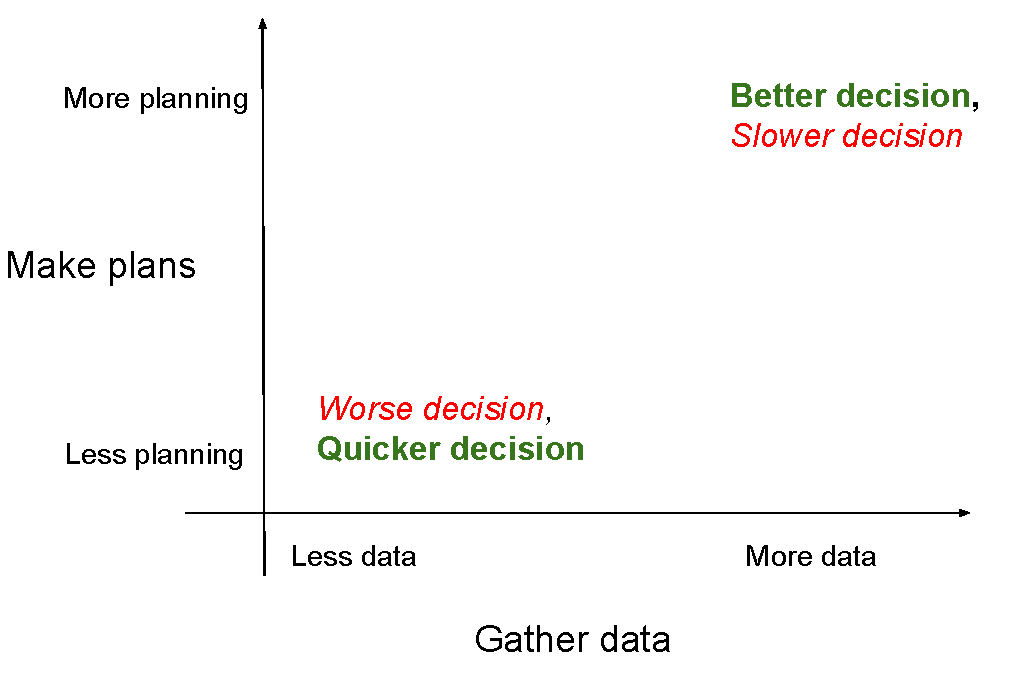
\includegraphics[width=0.8\textwidth]{images/planning_and_data_gathering.pdf}
    \caption{Planning (Dilemma~\ref{table:planning}) and data gathering (Dilemma~\ref{table:gather_data_lots-vs-little}) trade-off.}
    \label{fig:pareto_frontier}
\end{figure}

In practice, gathering data and planning rarely terminate -- they evolve.

% How does this relate directly to bureaucracy as defined as shared resource management policymaking?
The \href{table:opposition}{Dilemma of Disagreement}
% How does this impact your relationships with other bureaucrats?
The \href{table:opposition}{Dilemma of Disagreement}
% Are the incentive structures aligned to support one direction or the other?



When planning (Dilemma~\ref{table:planning}), aspects to consider include
%\begin{itemize}
%    \item 
the amount of risk seeking or tolerance (Dilemma~\ref{table:risk})
and
%    \item 
the intended scope of impact  (Dilemma~\ref{table:scope_broad-vs-narrow}).
%\end{itemize}

\begin{center}
\begin{table}[H] % ht
\begin{tabular}{ | m{\dilemmatablewidth}| m{\dilemmatablewidth} | } 
  \hline
  \textbf{Take on big risks and big rewards.} & 
  \textbf{Take on small risks and small rewards.} \\ 
  \hline
  \textit{Description}: High risk tolerance. &
  \textit{Description}: Low risk tolerance. \\
  \hline
  \textit{Pros}: Potential for failure and harm is significant. &
  \textit{Pros}: If any one investment fails, you can continue other efforts. \\
  \hline
  \textit{Cons}: Costly investment, longer feedback cycle. & 
  \textit{Cons}: Incremental can be slower. \\
  \hline
\end{tabular}
\caption{
\textit{Dilemma of \href{https://en.wikipedia.org/wiki/Risk_assessment}{Risk tolerance}.} 
\index{dilemma!of \href{https://en.wikipedia.org/wiki/Risk_assessment}{Risk tolerance}}
%{\tiny Tag: Personal choice.}
}
\label{table:risk}
\end{table}
\end{center}

% How does this relate directly to bureaucracy as defined as shared resource management policymaking?
The \href{table:risk}{Dilemma of Risk Tolerance}
% How does this impact your relationships with other bureaucrats?
The \href{table:risk}{Dilemma of Risk Tolerance}
% Are the incentive structures aligned to support one direction or the other?


\begin{center}
\begin{table}[H] % ht
\begin{tabular}{ | m{\dilemmatablewidth}| m{\dilemmatablewidth} | } 
  \hline
  \textbf{Broad scope of impact.} &
  \textbf{Narrow scope of impact.} \\
  \hline
  \textit{Description}: The consequence of the work has many stakeholders. &
  \textit{Description}: Small number of stakeholders. \\  
  \hline
  \textit{Pros}: Benefit more people. &
  \textit{Pros}: Niche impact means less dependencies on other people. \\
  \hline
  \textit{Cons}: Harder to get everyone in agreement. & 
  \textit{Cons}: Less visibility to the rest of the organization. \\
  \hline
\end{tabular}
\caption{
\textit{Dilemma of Scope of Impact.}
\index{dilemma!of scope of impact}
Scope of impact of your work. 
%{\tiny Tag: Personal choice}
}
\end{table}
\label{table:scope_broad-vs-narrow}
\end{center}

% How does this relate directly to bureaucracy as defined as shared resource management policymaking?
The \href{table:scope_broad-vs-narrow}{Dilemma of Scope of Impact}
% How does this impact your relationships with other bureaucrats?
The \href{table:scope_broad-vs-narrow}{Dilemma of Scope of Impact}
% Are the incentive structures aligned to support one direction or the other?


Once data is gathered (Dilemma~\ref{table:gather_data_lots-vs-little}) and a plan is made (Dilemma~\ref{table:planning}), the result is disseminated. The choice on how to disseminate is Dilemma~\ref{table:consistency} and Dilemma~\ref{table:disseminate_one-by-one}.

\begin{center}
\begin{table}[H] % ht
\begin{tabular}{ | m{\dilemmatablewidth}| m{\dilemmatablewidth} | } 
  \hline
  \textbf{Guidance updated often; Incremental change.} & 
  \textbf{Consistent application of policy over time. Rules persist; then sudden drastic change.} \\ 
  \hline
  \textit{Pros}: Adapt policy to new information and changing conditions. &
  \textit{Pros}: Stability is easier to predict between regime changes.  \\
  \hline
  \textit{Cons}: More work needed. Accused of lacking stability. & 
  \textit{Cons}: Doesn't adapt as conditions change. Accused of being inflexible to evolving conditions. \\
  \hline
\end{tabular}
\caption{
\textit{Dilemma of Consistency over time.} 
\index{dilemma!of consistency over time}
Stability of rules; how change is implemented. Can also be characterized as when to tell other people: sooner or later (when firmer information is available).
See the description of 
\hyperref[sec:static-dynamic-processes]{static versus dynamic processes}.
%\ifpageref
%on page~\pageref{sec:static-dynamic-processes}
%\fi
%\iftoggle{pageref}{%
%on page~\pageref{sec:static-dynamic-processes}
%}
%\iftoggle{sectionref}{%
%in section~\ref{sec:static-dynamic-processes} 
%}
%{\tiny Tag: Organization's culture. Tag: Personal choice.}
}
\label{table:consistency}
\end{table}
\end{center}

Deployment of products and deployment of policies face similar dilemmas. \href{https://en.wikipedia.org/wiki/Diffusion_of_innovations}{Diffusion of Innovation}.

% How does this relate directly to bureaucracy as defined as shared resource management policymaking?
The \href{table:consistency}{Dilemma of Consistency over time}
% How does this impact your relationships with other bureaucrats?
The \href{table:consistency}{Dilemma of Consistency over time}
% Are the incentive structures aligned to support one direction or the other?


\begin{center}
\begin{table}[H] % ht
\begin{tabular}{ | m{\dilemmatablewidth}| m{\dilemmatablewidth} | } 
  \hline
  \textbf{Tell people one-by-one.} & 
  \textbf{Tell everyone at once.} \\ 
  \hline
  \textit{Pros}: One-on-one allows a freer response from audience. &
  \textit{Pros}: Save time for the speaker. \\
  \hline
  \textit{Cons}: Order matters for relationships. & 
  \textit{Cons}: Overwhelming feedback all at once. \\  
  \hline
\end{tabular}
\caption{
\textit{Dilemma of Disseminating information.}
\index{dilemma!of disseminating information}
%{\tiny Tag: Personal choice.}
}
\label{table:disseminate_one-by-one}
\end{table}
\end{center}

Once a decision has been made, the decision is executed or enforced. How many rules are there (Dilemma~\ref{table:number_of_rules}) and
how strictly are the rules enforced (Dilemma~\ref{table:rule_strictness})?

% How does this relate directly to bureaucracy as defined as shared resource management policymaking?
The \href{table:disseminate_one-by-one}{Dilemma of Disseminating information}
% How does this impact your relationships with other bureaucrats?
The \href{table:disseminate_one-by-one}{Dilemma of Disseminating information}
% Are the incentive structures aligned to support one direction or the other?


\begin{center}
\begin{table}[H] % ht
\begin{tabular}{ | m{\dilemmatablewidth}| m{\dilemmatablewidth} | } 
  \hline
  \textbf{Enforce rules strictly.} & 
  \textbf{Lax rule enforcement.} \\ 
  \hline
  \textit{Pros}: Predictable. &
  \textit{Pros}: Bureaucrats feel empowered. \\
  \hline
  \textit{Cons}: Insensitive to nuance. & 
  \textit{Cons}: Tolerance for changing conditions or exceptional cases.  \\  
  \hline
\end{tabular}
\caption{
\textit{Dilemma of Strictness of rules.}
\index{dilemma!of strictness of rules}
%{\tiny Tag: Organization's culture.}
}
\label{table:rule_strictness}
\end{table}
\end{center}

% How does this relate directly to bureaucracy as defined as shared resource management policymaking?
The \href{table:rule_strictness}{Dilemma of Strictness of rules}
% How does this impact your relationships with other bureaucrats?
The \href{table:rule_strictness}{Dilemma of Strictness of rules}
% Are the incentive structures aligned to support one direction or the other?


\begin{center}
\begin{table}[H] % ht
\begin{tabular}{ | m{\dilemmatablewidth}| m{\dilemmatablewidth} | } 
  \hline
  \textbf{If it's not against the rules, it must be okay.} & 
  \textbf{I can only do what is allowed by the rules and nothing more.} \\ 
  \hline
  \textit{Pros}: Autonomy &
  \textit{Pros}:  \\
  \hline
  \textit{Cons}: . & 
  \textit{Cons}: .  \\  
  \hline
\end{tabular}
\caption{
\textit{Dilemma of Adherence to rules.}
\index{dilemma!of adherence to rules}
}
\label{table:rule_adherence}
\end{table}
\end{center}


% How does this relate directly to bureaucracy as defined as shared resource management policymaking?
The \href{table:rule_adherence}{Dilemma of Adherence to rules}
% How does this impact your relationships with other bureaucrats?
The \href{table:rule_adherence}{Dilemma of Adherence to rules}
% Are the incentive structures aligned to support one direction or the other?



\begin{center}
\begin{table}[H] % ht
\begin{tabular}{ | m{\dilemmatablewidth}| m{\dilemmatablewidth} | } 
  \hline
  \textbf{Control via rules.} & \textbf{Freedom/autonomy/agility.} \\ 
  \hline
  \textit{Description}: High number of rules to cover a variety of situations. & 
  \textit{Description}: Low number of rules to enable flexibility. \\ 
  \hline
  \textit{Cons}: The more rules that exist the more likely it is that someone will find a way to exploit them to their own advantage. & 
  \textit{Cons}: The fewer rules that exist the more likely it is that someone will try to get away with something bad. \\  
  \hline
\end{tabular}
\caption{
\textit{Dilemma of Number of rules.}
\index{dilemma!of number of rules}
%{\tiny Tag: Organization's culture}
}
\label{table:number_of_rules}
\end{table}
\end{center}
Alternative approach: guidance derived from principles that can be adapted to specific situations. That has the problem of requiring good knowledge of the situation and wise judgement.

% How does this relate directly to bureaucracy as defined as shared resource management policymaking?
The \href{table:number_of_rules}{Dilemma of Number of rules}
% How does this impact your relationships with other bureaucrats?
The \href{table:number_of_rules}{Dilemma of Number of rules}
% Are the incentive structures aligned to support one direction or the other?


\begin{center}
\begin{table}[H] % ht
\begin{tabular}{ | m{\dilemmatablewidth}| m{\dilemmatablewidth} | } 
  \hline
  \textbf{I can only do what is mandated by the organization.} & 
  \textbf{I can do anything that's not illegal.} \\ 
  \hline
  \textit{Cons}: Responding to novel situations is inhibited. &
  \textit{Cons}:  \\  
  \hline
\end{tabular}
\caption{
\textit{Dilemma of Legality.}
\index{dilemma!of legality}
The scope of your actions bound by mandates and legality, but the way you interpret that is subjective.
}
\label{table:legality}
\end{table}
\end{center}

% How does this relate directly to bureaucracy as defined as shared resource management policymaking?
The \href{table:legality}{Dilemma of Legality}
% How does this impact your relationships with other bureaucrats?
The \href{table:legality}{Dilemma of Legality}
% Are the incentive structures aligned to support one direction or the other?


\begin{center}
\begin{table}[H] % ht
\begin{tabular}{ | m{\dilemmatablewidth}| m{\dilemmatablewidth} | } 
  \hline
  \textbf{Decision in a process informed by a single bit of information.} & 
  \textbf{Fault tolerant decision making through redundancy.} \\ 
  \hline
  \textit{Cons}: Might be accidentally wrong. &
  \textit{Cons}: Extra burden of collecting and processing more data. \\  
  \hline
\end{tabular}
\caption{
\textit{Dilemma of Data for Decisions.}
\index{dilemma!of data for decisions}
Having a single checkmark on a form makes data collection easier. The person using the form might not see the checkmark box or may accidentally fill in the checkmark. The process is sensitive to this single bit of data.
}
\label{table:single-bit-decision}
\end{table}
\end{center}

% How does this relate directly to bureaucracy as defined as shared resource management policymaking?
The \href{table:single-bit-decision}{Dilemma of Data for Decisions}
% How does this impact your relationships with other bureaucrats?
The \href{table:single-bit-decision}{Dilemma of Data for Decisions}
% Are the incentive structures aligned to support one direction or the other?

\begin{center}
\begin{table}[H] % ht
\begin{tabular}{ | m{\dilemmatablewidth}| m{\dilemmatablewidth} | } 
  \hline
  \textbf{Quickly complete tasks or deploy new policies or create new products.} & 
  \textbf{Methodically complete tasks (or well-founded policies, quality products).} \\ 
  \hline
  \textit{Description}: Implement a solution quickly to address urgent needs. &
  \textit{Description}: Methodical well-planned design and execution yield robust solutions/products/policies. \\
  \hline
  \textit{Pros}: Rapid solution. &
  \textit{Pros}: More like to get the solution right. \\
  \hline
  \textit{Cons}: Risk of quick task is that the result is ineffective, inefficient, or wrong. &
  \textit{Cons}: \href{https://en.wikipedia.org/wiki/Opportunity_cost}{opportunity cost} \\  
  \hline
\end{tabular}
\caption{
\textit{Dilemma of Speed and Accuracy.}
\index{dilemma!of speed and accuracy}
Speed versus accuracy of task completion.
}
\label{table:quick-methodical}
\end{table}
\end{center}

If you try to resolve Dilemma~\ref{table:quick-methodical} by both getting a solution deployed quickly and then iterating towards a robust outcome, you may appear unpredictable or unstable; see Dilemma~\ref{table:planning}. This is an example of cascading dilemmas. The interplay of a creative resolution to one dilemma can impact the solution space for other dilemmas. 

% How does this relate directly to bureaucracy as defined as shared resource management policymaking?
The \href{table:quick-methodical}{Dilemma of Speed and Accuracy}
% How does this impact your relationships with other bureaucrats?
The \href{table:quick-methodical}{Dilemma of Speed and Accuracy}
% Are the incentive structures aligned to support one direction or the other?


\begin{center}
\begin{table}[H] % ht
\begin{tabular}{ | m{\dilemmatablewidth}| m{\dilemmatablewidth} | } 
  \hline
  \textbf{Push people to work really hard.} & 
  \textbf{Create a comfortable work environment.} \\ 
  \hline
  \textit{Cons}: Burn out and leave. & 
  \textit{Cons}: Lower instantaneous productivity. \\  
  \hline
\end{tabular}
\caption{
\textit{Dilemma of Urgency.}
\index{dilemma!of urgency}
}
\label{table:rate-of-work}
\end{table}
\end{center}

% How does this relate directly to bureaucracy as defined as shared resource management policymaking?
The \href{table:rate-of-work}{Dilemma of Urgency}
% How does this impact your relationships with other bureaucrats?
The \href{table:rate-of-work}{Dilemma of Urgency}
% Are the incentive structures aligned to support one direction or the other?


% https://bennorthrop.com/Essays/2022/code-ownership-stewardship-or-free-for-all.php
\begin{center}
\begin{table}[H] % ht
\begin{tabular}{ | m{\dilemmatablewidth}| m{\dilemmatablewidth} | } 
  \hline
  \textbf{Talk more to convey more information.} & 
  \textbf{Listen more to learn more information.} \\ 
  \hline
  \textit{Cons}: Less time available for listening. & 
  \textit{Cons}: Less time to convey what you know. \\  
  \hline
\end{tabular}
\caption{
\textit{Dilemma of Talking.}
\index{dilemma!of talking}
In conversations or meetings there is a (subjective) balance for participants.
}
\label{table:talk-or-listen}
\end{table}
\end{center}

% How does this relate directly to bureaucracy as defined as shared resource management policymaking?
The \href{table:talk-or-listen}{Dilemma of Talking}
% How does this impact your relationships with other bureaucrats?
The \href{table:talk-or-listen}{Dilemma of Talking}
% Are the incentive structures aligned to support one direction or the other?



\begin{center}
\begin{table}[H] % ht
\begin{tabular}{ | m{\dilemmatablewidth}| m{\dilemmatablewidth} | } 
  \hline
  \textbf{Seek out experienced collaborators.} & 
  \textbf{Work with less experienced people.} \\ 
  \hline
  \textit{Pros}: Quicker to get something done. &
  \textit{Pros}: Less set in their ways and open to more novelty. \\  
  \hline
  \textit{Cons}: Experienced people who are good are probably busy. &
  \textit{Cons}: Slower progress. \\  
  \hline
\end{tabular}
\caption{
\textit{Dilemma of Experienced Collaborators.}
\index{dilemma!of experienced collaborators}
People with experience are useful but less accessible.
}
\label{table:experience}
\end{table}
\end{center}


% How does this relate directly to bureaucracy as defined as shared resource management policymaking?
The \href{table:experience}{Dilemma of Experienced Collaborators}
% How does this impact your relationships with other bureaucrats?
The \href{table:experience}{Dilemma of Experienced Collaborators}
% Are the incentive structures aligned to support one direction or the other?


\begin{center}
\begin{table}[H] % ht
\begin{tabular}{ | m{\dilemmatablewidth}| m{\dilemmatablewidth} | } 
  \hline
  \textbf{Say yes to new opportunities.} & 
  \textbf{Say no to new opportunities.} \\ 
  \hline
  \textit{Pros}: Positive attitude, collaborative. &
  \textit{Pros}: Able to prioritize and focus. \\
  \hline
  \textit{Cons}: Fail to complete tasks. &
  \textit{Cons}: Not a team player. \\  
  \hline
\end{tabular}
\caption{
\textit{Dilemma of opportunities.}
\index{dilemma!of opportunities}
Acceptance or rejection of additional work can be explicit or implicit. Bureaucrats respond to this challenge by sending mixed signals: expressing interest but not following up with action.
}
\label{table:new-opportunties}
\end{table}
\end{center}

% How does this relate directly to bureaucracy as defined as shared resource management policymaking?
The \href{table:new-opportunties}{Dilemma of opportunities}
% How does this impact your relationships with other bureaucrats?
The \href{table:new-opportunties}{Dilemma of opportunities}
% Are the incentive structures aligned to support one direction or the other?


\begin{center}
\begin{table}[H] % ht
\begin{tabular}{ | m{\dilemmatablewidth}| m{\dilemmatablewidth} | } 
  \hline
  \textbf{Share less data.} &
  \textbf{Share more data.} \\
%  \hline
%  \textit{Description}:  &
%  \textit{Description}:  \\  
  \hline
  \textit{Pros}: Restricting data access saves money for the data owner.&
  \textit{Pros}: Sharing data improves transparency and accountability. \\
  \hline
  \textit{Cons}: People other than the data owner are unable to extract value from data. & 
  \textit{Cons}: Sharing data uses resources (people, money, time). \\
  \hline
\end{tabular}
\caption{
\textit{Dilemma of Sharing Data.}
\index{dilemma!of sharing data}
How much data to share. Potential solution is to make data discoverable. Advertise the availability of data without providing data. This way a negotiation is feasible for people interested in the data.
%{\tiny Tag: Personal choice.}
}
\label{table:data_share-vs-hide}
\end{table}
\end{center}

In \ref{table:data_share-vs-hide} there is a lot of aspects of data than can be shared for discoverability: who to contact about access, what the data sources are, how often data is collected, how long data is stored, how much data there is.

% How does this relate directly to bureaucracy as defined as shared resource management policymaking?
The \href{table:data_share-vs-hide}{Dilemma of Sharing Data}
% How does this impact your relationships with other bureaucrats?
The \href{table:data_share-vs-hide}{Dilemma of Sharing Data}
% Are the incentive structures aligned to support one direction or the other?


\begin{center}
\begin{table}[H] % ht
\begin{tabular}{ | m{\dilemmatablewidth}| m{\dilemmatablewidth} | } 
  \hline
  \textbf{Compete for resources.} &
  \textbf{Cooperate for productivity.} \\
  \hline
  \textit{Description}: individuals compete for attention and promotion; teams compete for money and staffing resources &
  \textit{Description}: cooperation improves productivity \\  
  \hline
  \textit{Cons}: Fail to synergize skills resources & 
  \textit{Cons}: Not clear who to assign responsibility for success or failure \\
  \hline
\end{tabular}
\caption{
\textit{Dilemma of Cooperate or Compete.} 
\index{dilemma!of cooperate or compete}
Applies to teams and to individuals. 
%{\tiny Tag: Personal choice.}
}
\label{table:cooperate-vs-compete}
\end{table}
\end{center}

% How does this relate directly to bureaucracy as defined as shared resource management policymaking?
The \href{table:cooperate-vs-compete}{Dilemma of Cooperate or Compete}
% How does this impact your relationships with other bureaucrats?
The \href{table:cooperate-vs-compete}{Dilemma of Cooperate or Compete}
% Are the incentive structures aligned to support one direction or the other?


\begin{center}
\begin{table}[H] % ht
\begin{tabular}{ | m{\dilemmatablewidth}| m{\dilemmatablewidth} | }
  \hline
  \textbf{Consistent application of policy across cases.} &
  \textbf{Adapt policy to specific cases.} \\
  \hline
  \textit{Description}: Maximize broad applicability; minimize exceptions. &
  \textit{Description}: Demonstrate flexibility for unique scenarios. \\  
  \hline
  \textit{Cons}: Less sensitive to the nuances of a specific situation. & 
  \textit{Cons}: Takes more work. More likely to be accused of bias. \\
  \hline
\end{tabular}
\caption{
\textit{Dilemma of Consistent Policies.}
\index{dilemma!of consistency policies}
Case consistency vs adaptability.
%{\tiny Tag: Personal choice.}
}
\label{table:policy_consistency_across_cases}
\end{table}
\end{center}

When change to policies is desired, there are options on how to advocate for change -- Dilemma~\ref{table:how_to_change}.

% How does this relate directly to bureaucracy as defined as shared resource management policymaking?
The \href{table:policy_consistency_across_cases}{Dilemma of Consistent Policies}
% How does this impact your relationships with other bureaucrats?
The \href{table:policy_consistency_across_cases}{Dilemma of Consistent Policies}
% Are the incentive structures aligned to support one direction or the other?


% https://bennorthrop.com/Essays/2022/code-ownership-stewardship-or-free-for-all.php
\begin{center}
\begin{table}[H] % ht
\begin{tabular}{ | m{\dilemmatablewidth}| m{\dilemmatablewidth} | } 
  \hline
  \textbf{One person or team owns an area of responsibility.} & 
  \textbf{Anyone take on any task.} \\ 
  \hline
  \textit{Cons}: Staffing capacity may not be as flexible as varying workload. & 
  \textit{Cons}: Not everyone is skilled at everything. \\  
  \hline
\end{tabular}
\caption{
\textit{Dilemma of Swimlanes.} 
\index{dilemma!of swimlanes}
How are tasks assigned? This can be negotiated with coworkers and is not intrinsic to structure of the organization. 
}
\label{table:swimlanes}
\end{table}
\end{center}


Independent of how tasks are assigned within a team or organization (Dilemma~\ref{table:swimlanes}), individual bureaucrats can decide how they act in Dilemma~\ref{table:scope_of_activity}.


% How does this relate directly to bureaucracy as defined as shared resource management policymaking?
The \href{table:swimlanes}{Dilemma of Swimlanes}
% How does this impact your relationships with other bureaucrats?
The \href{table:swimlanes}{Dilemma of Swimlanes}
% Are the incentive structures aligned to support one direction or the other?


\begin{center}
\begin{table}[H] % ht
\begin{tabular}{ | m{\dilemmatablewidth}| m{\dilemmatablewidth} | }
  \hline
% https://graphthinking.blogspot.com/2019/07/not-too-loose-not-too-tight-determining.html
  \textbf{Adhere strictly to the scope of your role.} & 
  \textbf{Stray outside (or outright ignore) the scope of your role.} \\ 
  \hline
  \textit{Description}: Inflexible to novelty. Specialization of tasking. & 
  \textit{Description}: Lack of structure. Generalization. \\ 
  \hline
  \textit{Cons}: Efficiencies of cooperation and specialization would not occur. & 
  \textit{Cons}: \href{https://en.wikipedia.org/wiki/Deadlock}{Deadlock} condition arises due to a scheduling constraint -- no one can proceed because everyone is waiting on everyone else. Responsibilities are unclear when no ones scope is clear. \\  
  \hline
\end{tabular}
\caption{
\textit{Dilemma of Scope.}
\index{dilemma!of scope}
Both strict adherence to role scope and ignoring scope can decrease an organization's productivity. 
What happens when a person deviates from their role?
How are people who do not conform identified? Are they confronted?
}
\label{table:scope_of_activity}
\end{table}
\end{center}


% How does this relate directly to bureaucracy as defined as shared resource management policymaking?
The \href{table:scope_of_activity}{Dilemma of Scope}
% How does this impact your relationships with other bureaucrats?
The \href{table:scope_of_activity}{Dilemma of Scope}
% Are the incentive structures aligned to support one direction or the other?


\begin{center}
\begin{table}[H] % ht
\begin{tabular}{ | m{\dilemmatablewidth}| m{\dilemmatablewidth} | } 
  \hline
  \textbf{Delegate; share work with other people.} & 
  \textbf{Work alone; don't rely on other people.} \\ 
  \hline
  \textit{Cons}: Your success is dependent on other people. & 
  \textit{Cons}: Can't do as much on your own. \\  
  \hline
\end{tabular}
\caption{
\textit{Dilemma of Delegation.}
\index{dilemma!of delegation}
Sharing work can improve productivity and build relationships but also incurs risks to reputation and success.
}
\label{table:delegate-or-not}
\end{table}
\end{center}


% How does this relate directly to bureaucracy as defined as shared resource management policymaking?
The \href{table:delegate-or-not}{Dilemma of Delegation}
% How does this impact your relationships with other bureaucrats?
The \href{table:delegate-or-not}{Dilemma of Delegation}
% Are the incentive structures aligned to support one direction or the other?


\begin{center}
\begin{table}[H] % ht
\begin{tabular}{ | m{\dilemmatablewidth}| m{\dilemmatablewidth} | } 
  \hline
  \textbf{Health of the organization.} & 
  \textbf{Results of the organization.} \\ 
  \hline
  \textit{Description}: Maintain processes and train staff. Considered ``overhead.'' & 
  \textit{Description}: Do the work that motivates the existence of the organization. \\  
    \hline
  \textit{Cons}: Unproductive for subjects. & 
  \textit{Cons}: Unsustainable for members. \\
  \hline
\end{tabular}
\caption{
\textit{Dilemma of Health versus Results.}
\index{dilemma!of health versus results}
 Producing the results that motivated the existence of an organization often requires spending organization's health
}
\label{table:health-vs-results}
\end{table}
\end{center}

% How does this relate directly to bureaucracy as defined as shared resource management policymaking?
The \href{table:health-vs-results}{Dilemma of Health versus Results}
% How does this impact your relationships with other bureaucrats?
The \href{table:health-vs-results}{Dilemma of Health versus Results}
% Are the incentive structures aligned to support one direction or the other?

\begin{center}
\begin{table}[H] % ht
\begin{tabular}{ | m{\dilemmatablewidth}| m{\dilemmatablewidth} | } 
  \hline
  \textbf{Many small tasks or goals.} & 
  \textbf{Fewer big tasks or goals.} \\ 
  \hline
  \textit{Description}: Your day is occupied with a variety of short-duration tasks. & 
  \textit{Description}: You work on only a few efforts during a typical day. \\  
    \hline
  \textit{Cons}: Enables a fail fast approach from quick feedback. & 
  \textit{Cons}: Less overhead of task switching to manage. \\
  \hline
\end{tabular}
\caption{
\textit{Dilemma of Chunk size.}
\index{dilemma!of chunk size}
You may or may not have a choice of task size and number of tasks. If you have autonomy, what do you prefer? Do your coworkers and supervisors know your preference? 
}
\label{table:chunk_size}
\end{table}
\end{center}


% How does this relate directly to bureaucracy as defined as shared resource management policymaking?
The \href{table:chunk_size}{Dilemma of Chunk size}
% How does this impact your relationships with other bureaucrats?
The \href{table:chunk_size}{Dilemma of Chunk size}
% Are the incentive structures aligned to support one direction or the other?


\begin{center}
\begin{table}[H] % ht
\begin{tabular}{ | m{\dilemmatablewidth}| m{\dilemmatablewidth} | } 
  \hline
  \textbf{Task with many external dependencies.} & 
  \textbf{Task with few external dependencies.} \\ 
  \hline
  \textit{Cons}: Risk of failing because of a failed dependency. & 
  \textit{Cons}: Have to develop everything yourself; waste of resources due to redundancy. \\  
  \hline
\end{tabular}
\caption{
\textit{Dilemma of Dependencies.}
\index{dilemma!of dependencies}
External dependencies can enable broader scope. This Dilemma only is relevant if you have autonomy in the selection of your tasks. See also the Dilemma of Delegation, \ref{table:delegate-or-not}.
}
\label{table:number_of_external dependencies}
\end{table}
\end{center}


% How does this relate directly to bureaucracy as defined as shared resource management policymaking?
The \href{table:number_of_external dependencies}{Dilemma of Dependencies}
% How does this impact your relationships with other bureaucrats?
The \href{table:number_of_external dependencies}{Dilemma of Dependencies}
% Are the incentive structures aligned to support one direction or the other?


\begin{center}
\begin{table}[H] % ht
\begin{tabular}{ | m{\dilemmatablewidth}| m{\dilemmatablewidth} | } 
  \hline
  \textbf{Focused on one role.} & 
  \textbf{Have multiple roles.} \\ 
  \hline
  \textit{Cons}: If a role does not consume 40 hours per week, you'll be idle. & 
  \textit{Cons}: Context switches between roles and delayed responses. \\  
  \hline
\end{tabular}
\caption{
\textit{Dilemma of Roles.}
\index{dilemma!of roles}
The right number of roles for a bureaucrat depends on personality and tasking. 
}
\label{table:number_of_roles}
\end{table}
\end{center}


% How does this relate directly to bureaucracy as defined as shared resource management policymaking?
The \href{table:number_of_roles}{Dilemma of Roles}
% How does this impact your relationships with other bureaucrats?
The \href{table:number_of_roles}{Dilemma of Roles}
% Are the incentive structures aligned to support one direction or the other?


\begin{center}
\begin{table}[H] % ht
\begin{tabular}{ | m{\dilemmatablewidth}| m{\dilemmatablewidth} | } 
  \hline
  \textbf{Dissent is welcome and discussed freely.} & 
  \textbf{Dissent is suppressed.} \\ 
  \hline
  \textit{Cons}: Can be disruptive to normal operations. Distracts from the task. & 
  \textit{Cons}: Limits novel ideas from spreading. Harms morale. \\  
  \hline
\end{tabular}
\caption{
\textit{Dilemma of Dissent.}
\index{dilemma!of dissent}
Dissent is caused by dissatisfaction with people or processes. 
}
\label{table:how_dissent_is_responded_to}
\end{table}
\end{center}


% How does this relate directly to bureaucracy as defined as shared resource management policymaking?
The \href{table:how_dissent_is_responded_to}{Dilemma of Dissent}
% How does this impact your relationships with other bureaucrats?
The \href{table:how_dissent_is_responded_to}{Dilemma of Dissent}
% Are the incentive structures aligned to support one direction or the other?


\begin{center}
\begin{table}[H] % ht
\begin{tabular}{ | m{\dilemmatablewidth}| m{\dilemmatablewidth} | } 
  \hline
  \textbf{Do share lessons learned.} & 
  \textbf{Don't share lessons learned.} \\ 
  \hline
  \textit{Pros}: Honesty, accountability, self-awareness, and self-reflection. & 
  \textit{Pros}: Look competent, even when making mistakes. \\  
  \hline
  \textit{Cons}: Looks weak, unprofessional. & 
  \textit{Cons}: Limit the growth of bureaucrats in the organization. \\  
  \hline
\end{tabular}
\caption{
\textit{Dilemma of Sharing Lessons.}
\index{dilemma!of sharing lessons}
Sharing lessons learned may seem reasonable unless you want to maintain a pristine reputation. 
}
\label{table:sharing_lessons_learned}
\end{table}
\end{center}


% How does this relate directly to bureaucracy as defined as shared resource management policymaking?
The \href{table:sharing_lessons_learned}{Dilemma of Sharing Lessons}
% How does this impact your relationships with other bureaucrats?
The \href{table:sharing_lessons_learned}{Dilemma of Sharing Lessons}
% Are the incentive structures aligned to support one direction or the other?


% https://graphthinking.blogspot.com/2019/07/vulnerability-of-organizations-in.html
\begin{center}
\begin{table}[H] % ht
\begin{tabular}{ | m{\dilemmatablewidth}| m{\dilemmatablewidth} | } 
  \hline
  \textbf{Share lessons learned about yourself.} & 
  \textbf{Share lessons learned from observing others.} \\ 
  \hline
  \textit{Cons}: Potentially look stupid. & 
  \textit{Cons}: Potentially hurts their reputation. \\  
  \hline
\end{tabular}
\caption{
\textit{Dilemma of Sharing.}
\index{dilemma!of sharing}
When sharing lessons learned (option 1 in \ref{table:sharing_lessons_learned}), the lessons do not have to be about you. 
}
\label{table:share_lessons_learned}
\end{table}
\end{center}


% How does this relate directly to bureaucracy as defined as shared resource management policymaking?
The \href{table:share_lessons_learned}{Dilemma of Sharing}
% How does this impact your relationships with other bureaucrats?
The \href{table:share_lessons_learned}{Dilemma of Sharing}
% Are the incentive structures aligned to support one direction or the other?


\begin{center}
\begin{table}[H] % ht
\begin{tabular}{ | m{\dilemmatablewidth}| m{\dilemmatablewidth} | } 
  \hline
  \textbf{Learn lessons from your own mistakes.} & 
  \textbf{Learn lessons from others (formal training).} \\ 
  \hline
  \textit{Cons}: Potentially look stupid; waste resources discovering what others already know. & 
  \textit{Cons}: Formal training may overemphasize irrelevant or impractical concepts. \\  
  \hline
\end{tabular}
\caption{
\textit{Dilemma of Learning.}
\index{dilemma!of learning}
How much formal training to invest in before learning by doing?
}
\label{table:lessons_learned_source}
\end{table}
\end{center}


% How does this relate directly to bureaucracy as defined as shared resource management policymaking?
The \href{table:lessons_learned_source}{Dilemma of Learning}
% How does this impact your relationships with other bureaucrats?
The \href{table:lessons_learned_source}{Dilemma of Learning}
% Are the incentive structures aligned to support one direction or the other?


\begin{center}
\begin{table}[H] % ht
\begin{tabular}{ | m{\dilemmatablewidth}| m{\dilemmatablewidth} | } 
  \hline
  \textbf{Build a small coalition of interested parties.} & 
  \textbf{Build a large base of support and get everyone on board.} \\ 
  \hline
  \textit{Cons}: May not be representative of all stakeholders. & 
  \textit{Cons}: Takes time away from the work. Many people may disagree or be disinterested. \\  
  \hline
\end{tabular}
\caption{
\textit{Dilemma of Coalitions.}
\index{dilemma!of coalitions}
A coalition can provide morale support but takes time to build.
%{\tiny Tag: }
}
\label{table:how_to_change}
\end{table}
\end{center}


% How does this relate directly to bureaucracy as defined as shared resource management policymaking?
The \href{table:how_to_change}{Dilemma of Coalitions}
% How does this impact your relationships with other bureaucrats?
The \href{table:how_to_change}{Dilemma of Coalitions}
% Are the incentive structures aligned to support one direction or the other?


\begin{center}
\begin{table}[H] % ht
\begin{tabular}{ | m{\dilemmatablewidth}| m{\dilemmatablewidth} | } 
  \hline
  \textbf{Process request as they arrive.} &
  \textbf{Process request in batches.} \\
  \hline
%  \textit{Description}: . & 
%  \textit{Description}: . \\
%  \hline
  \textit{Pros}: Responsive. & 
  \textit{Pros}: Improves efficiency. \\
  \hline
  \textit{Cons}: Decreased efficiency. & 
  \textit{Cons}: Induces a delay in processing. \\
  \hline
\end{tabular}
\caption{
\textit{Dilemma of Batching.}
\index{dilemma!of batching}
For repeated actions, who is the process optimized for -- the subject or the bureaucrat?
}
\label{table:dilemma-of-batching}
\end{table}
\end{center}


% How does this relate directly to bureaucracy as defined as shared resource management policymaking?
The \href{table:dilemma-of-batching}{Dilemma of Batching}
% How does this impact your relationships with other bureaucrats?
The \href{table:dilemma-of-batching}{Dilemma of Batching}
% Are the incentive structures aligned to support one direction or the other?


\begin{center}
\begin{table}[H] % ht
\begin{tabular}{ | m{\dilemmatablewidth}| m{\dilemmatablewidth} | } 
  \hline
  \textbf{Redundant reviews of data.} &
  \textbf{Single review of data.} \\
  \hline
  \textit{Description}: Multiple independent confirmations that the data collected is correct. & 
  \textit{Description}: A form featuring a checkbox option.  \\
  \hline
  \textit{Pros}: Decrease mistakes. & 
  \textit{Pros}: Less overhead. \\
  \hline
  \textit{Cons}: More people or time needed. & 
  \textit{Cons}: Single point of failure. \\
  \hline
\end{tabular}
\caption{
\textit{Dilemma of Redundancy.}
\index{dilemma!of redundancy}
If a user doesn't see a checkbox on a form, or they incorrectly mark the checkbox, is there any validation of the selection?
}
\label{table:dilemma-of-redundancy}
\end{table}
\end{center}


% How does this relate directly to bureaucracy as defined as shared resource management policymaking?
The \href{table:dilemma-of-redundancy}{Dilemma of Redundancy}
% How does this impact your relationships with other bureaucrats?
The \href{table:dilemma-of-redundancy}{Dilemma of Redundancy}
% Are the incentive structures aligned to support one direction or the other?


\subsection*{Dilemmas of Policy for an Organization's Structure\label{sec:org-dilemma}}

The constraints a decision maker faces are informed by the person's environment. Dilemmas \ref{table:people-per-supervisor} through \ref{table:market-vs-monopoly} shape the experience of bureaucrats in an organization.

\begin{center}
\begin{table}[H] % ht
\begin{tabular}{ | m{\dilemmatablewidth}| m{\dilemmatablewidth} | } 
  \hline
  \textbf{Flatter hierarchical organization.} &
  \textbf{More layers of hierarchy.} \\ 
  \hline
  \textit{Description}: More people managed per supervisor. & 
  \textit{Description}: Fewer people managed per supervisor. \\ 
  \hline
  \textit{Cons}: Less feedback/attention per employee. & 
  \textit{Cons}: Fewer people doing work. \\  
  \hline
\end{tabular}
\caption{
\textit{Dilemma of Shape of hierarchical organization.}
\index{dilemma!of flatness}
%{\tiny Tag: Organization's culture}
}
\label{table:people-per-supervisor}
\end{table}
\end{center}


% How does this relate directly to bureaucracy as defined as shared resource management policymaking?
The \href{table:people-per-supervisor}{Dilemma of Shape of hierarchical organization}
% How does this impact your relationships with other bureaucrats?
The \href{table:people-per-supervisor}{Dilemma of Shape of hierarchical organization}
% Are the incentive structures aligned to support one direction or the other?


\begin{center}
\begin{table}[H] % ht
\begin{tabular}{ | m{\dilemmatablewidth}| m{\dilemmatablewidth} | } 
  \hline
  \textbf{Staffing: good coverage.} &
  \textbf{Staffing: minimal coverage.} \\
  \hline
  \textit{Description}: Sufficient staff. &
  \textit{Description}: As small of staff as possible. \\  
  \hline
  \textit{Pros}: Cover all edge cases; resilient to changing demands. &
  \textit{Pros}: Less expensive. \\
  \hline
  \textit{Cons}: Slack resources; sometimes inefficient. Increased communication needed. & 
  \textit{Cons}: Fragile when requirements change or workload increases. If one person leaves and there's no redundancy, capacity and capability are harmed.  \\
  \hline
\end{tabular}
\caption{
\textit{Dilemma of Size of team or organization.}
\index{dilemma!of team size}
%{\tiny Tag: Design of organization.}
}
\label{table:staff_many-vs-few}
\end{table}
\end{center}


% How does this relate directly to bureaucracy as defined as shared resource management policymaking?
The \href{table:staff_many-vs-few}{Dilemma of Size of team or organization}
% How does this impact your relationships with other bureaucrats?
The \href{table:staff_many-vs-few}{Dilemma of Size of team or organization}
% Are the incentive structures aligned to support one direction or the other?


\begin{center}
\begin{table}[H] % ht
\begin{tabular}{ | m{\dilemmatablewidth}| m{\dilemmatablewidth} | } 
  \hline
  \textbf{In-house services for non-central activities.} &
  \textbf{External dependencies for non-central activities.} \\
%  \hline
%  \textit{Description}:  &
%  \textit{Description}:  \\  
  \hline
  \textit{Pros}: More control. &
  \textit{Pros}: Easier to replace. \\
  \hline
  \textit{Cons}: Expands scope of responsibilities. & 
  \textit{Cons}: Less understanding of problem.  \\
  \hline
\end{tabular}
\caption{
\textit{Dilemma of Services.}
\index{dilemma!of services}
Services that are necessary but not central.
%{\tiny Tag: Design of organization.}
}
\label{table:inhouse-vs-external}
\end{table}
\end{center}

Table~\ref{table:inhouse-vs-external} isn't unique to bureaucracy. It applies to businesses in a market and to governments in a global environment. 


% How does this relate directly to bureaucracy as defined as shared resource management policymaking?
The \href{table:inhouse-vs-external}{Dilemma of Services}
% How does this impact your relationships with other bureaucrats?
The \href{table:inhouse-vs-external}{Dilemma of Services}
% Are the incentive structures aligned to support one direction or the other?


\begin{center}
\begin{table}[H] % ht
\begin{tabular}{ | m{\dilemmatablewidth}| m{\dilemmatablewidth} | } 
  \hline
  \textbf{Centralized services.} &
  \textbf{Locally distributed services.} \\
  \hline
  \textit{Description}: A single provider of services for the organization; typically top-down mandate. &
  \textit{Description}: Each team has a local service provider; typically bottom-up organic result. \\  
  \hline
  \textit{Pros}: Cheaper. Enables coordination. &
  \textit{Pros}: Quicker response. 
  Enables innovation. 
  Accounts for local deviations from the norm. \\
  \hline
  \textit{Cons}: Less sensitive to local issues. Less responsive. Longer delays. Single point of failure.  & 
  \textit{Cons}: Uneven quality of service. Inconsistent strategies and policies. \\
  \hline
\end{tabular}
\caption{
\textit{Dilemma of Centralization of Services.}
\index{dilemma!of centralization}
Oscillation (see figure\ref{fig:central-vs-distributed}) indicates neither solution is optimal.
%{\tiny Tag: Design of organization.}
}
\label{table:central-vs-distributed}
\end{table}
\end{center}

\begin{figure}[H] % ht
    \centering
    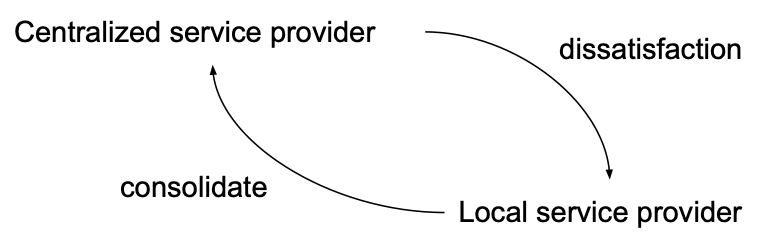
\includegraphics[width=0.8\textwidth]{images/dilemma_centralization-vs-distributed.pdf}
    \caption{Dipole oscillation. See Dilemma~\ref{table:central-vs-distributed}. Migrating to the opposite paradigm gives people in charge a chance to show their responsiveness to the needs of participants. The rate of oscillation is a measure of institutional memory half-life.}
    \label{fig:central-vs-distributed}
\end{figure}


% How does this relate directly to bureaucracy as defined as shared resource management policymaking?
The \href{table:central-vs-distributed}{Dilemma of Centralization of Services}
% How does this impact your relationships with other bureaucrats?
The \href{table:central-vs-distributed}{Dilemma of Centralization of Services}
% Are the incentive structures aligned to support one direction or the other?


Centralization is often carried out for the purposes of cost efficiency. The cost savings are due to de-duplication and having less slack. Both of those ``savings'' are a decrease of redundancy, which has a cost when there are unexpected fluctuations in need. 

Centralization is an intentional monopolization, with the corresponding decrease in choices. 
Centralization (de-localization) can decrease the value assigned to feedback from people using the service because personal relations are de-valued. 

The weaker feedback, lack of redundancy, and decreased emphasis on relationships motivates the creation of local services. 

\ \\

\begin{center}
\begin{table}[H] % ht
\begin{tabular}{ | m{\dilemmatablewidth}| m{\dilemmatablewidth} | } 
  \hline
  \textbf{Decision making lower in a hierarchy} &
  \textbf{Decision making higher in a hierarchy} \\
  \hline
  \textit{Description}: Push decisions down to empower employees. &
  \textit{Description}: Escalate every decision to management. \\  
  \hline
  \textit{Pros}: Better information. &
  \textit{Pros}: Better scope. \\
  \hline
  \textit{Cons}: more inconsistency & 
  \textit{Cons}: Decision maker has less skin in the game and may be less well informed. Employees are disempowered. \\
  \hline
\end{tabular}
\caption{
\textit{Dilemma of Decision height.}
\index{dilemma!of decision height}
Where decisions get made in hierarchical organization.
%{\tiny Tag: Design of organization.}
}
\label{table:decisions_low-vs-high}
\end{table}
\end{center}


% How does this relate directly to bureaucracy as defined as shared resource management policymaking?
The \href{table:decisions_low-vs-high}{Dilemma of Decision height}
% How does this impact your relationships with other bureaucrats?
The \href{table:decisions_low-vs-high}{Dilemma of Decision height}
% Are the incentive structures aligned to support one direction or the other?


\begin{center}
\begin{table}[H] % ht
\begin{tabular}{ | m{\dilemmatablewidth}| m{\dilemmatablewidth} | } 
  \hline
  \textbf{Redundant services in a market} &
  \textbf{Monopoly service provider} \\
  \hline
  \textit{Description}: using a market model within the organization &
  \textit{Description}:  \\  
  \hline
  \textit{Pros}: enable customers to choose the best service &
  \textit{Pros}: efficiency of a single service \\
  \hline
  \textit{Cons}: redundancy & 
  \textit{Cons}: might not meet the needs of all customers \\
  \hline
\end{tabular}
\caption{
\textit{Dilemma of Monopoly.}
\index{dilemma!of monopoly}
Services within an organization. See also figure\ref{fig:market-vs-monopoly}.
%{\tiny Tag: Design of organization.}
}
\label{table:market-vs-monopoly}
\end{table}
\end{center}


\begin{figure}[H] % ht
    \centering
    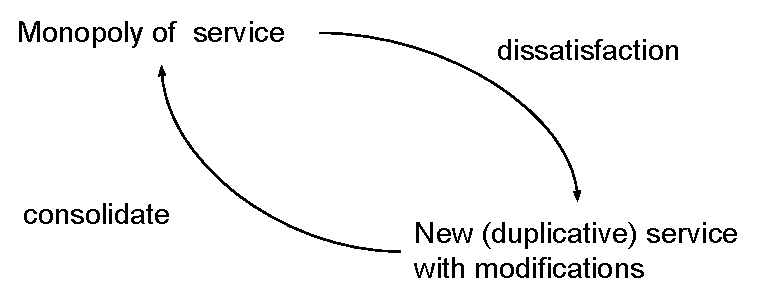
\includegraphics[width=0.8\textwidth]{images/dilemma_market_vs_monopoly.pdf}
    \caption{Dipole oscillation: solution A exists but doesn't meet my needs. Rather than tweak A, re-invent solution B which mostly overlaps with A but has independent development and support. See also Dilemma~\ref{table:market-vs-monopoly}.}
    \label{fig:market-vs-monopoly}
\end{figure}


% How does this relate directly to bureaucracy as defined as shared resource management policymaking?
The \href{table:market-vs-monopoly}{Dilemma of Monopoly}
% How does this impact your relationships with other bureaucrats?
The \href{table:market-vs-monopoly}{Dilemma of Monopoly}
% Are the incentive structures aligned to support one direction or the other?


% https://graphthinking.blogspot.com/2021/04/laffer-curve-and-minimum-viable.html
There is a Goldilocks situation for amount of processes in an organization:
\begin{itemize}
    \item Too few processes (all social relationships).
    \item Just the right amount -- a balance process and social, and when to use which is known.
    \item Too much process (not enough leveraging of social relationships)
\end{itemize}
This optimization is like the \href{https://en.wikipedia.org/wiki/Laffer_curve}{Laffer curve} in economics.

\ \\

\textit{Trilemma}: \textbf{Do you support the cutting edge, most of the middle, or the laggards?}\\
\index{trilemma!cutting edge, middle, laggards}
For any given aspect of bureaucracy there is a \href{https://en.wikipedia.org/wiki/Normal_distribution}{bell curve} of skills and interest of bureaucrats. In your role of bureaucrat you face a choice: find and collaborate with and enable the best and brightest, or aim your efforts at the massive mediocre middle (most bureaucrats), or try to get the dumbest bureaucrats up to speed? 

Trying to escape the trilemma by claiming that you treat everyone equally means you are disregarding the needs of the tail of the distribution. 

\ \\

% https://graphthinking.blogspot.com/2021/12/hierarchical-organization-trilemma.html
\textit{Trilemma}: \textbf{Do you work for your team, your manager, or yourself?} \\
\index{trilemma!team, manager, yourself}
Being a member of a team that operates within a hierarchy is tough. One reason is the question of who you are working for. The trilemma is whether you work for yourself, work for your supervisor, or work for your team.  Ideally you can find ways to do all three, but that is not always the case. 

Members of the team should work collaboratively, but there is a potential counter-force: accountability to the supervisor. Because each team member is accountable to their supervisor(s), that motivates the action of the individual. The team does not actually have autonomy -- they are accountable to the boss.

In the approach ``team members are directed by their supervisor," the synergy of the team is neglected and the supervisor becomes a bottleneck (for decision making and for creativity and for planning).

The third approach is for a person to ignore their team and their supervisor. This might enable quicker progress, at the risk of going in an unhelpful direction or not leveraging skills of coworkers. 

\ \\

\textit{Trilemma}:
\textbf{Seek less budget, same, or larger budget.} 
\index{trilemma!less, same, or larger budget}
Less budget is needed if you improved efficiency, but then the proportional power within the organization is decreased. A larger budget may be due to inefficiency or growth. Keeping the same budget indicates no promotions are relevant (although a steady state could result from a combination of growth and improved efficency). 

\ \\

A trilemma applicable to many situations is that options are \textbf{fast, inexpensive, good; choose two}. 
\index{trilemma!fast, inexpensive, good}
(This is the \href{https://en.wikipedia.org/wiki/Project_management_triangle}{Project management triangle}.) \\
\index{folk wisdom!\href{https://en.wikipedia.org/wiki/Project_management_triangle}{Project management triangle}}
In other words, the options are
\begin{itemize}
    \item Good and fast is expensive (i.e., requires lots of resources).
    \item Good and inexpensive takes a long time (i.e., find a clever solution).
    \item Fast and inexpensive will be low quality.
\end{itemize}

\subsection*{Dilemmas Raised by Subjects of Bureaucracy\label{sec:subjects-dilemmas}}

Each subject of bureaucracy views themselves as logical and self-consistent and erudite. In practice, the bureaucrat servicing subjects encounters conflicting statements. 

\begin{center}
\begin{table}[H] % ht
\begin{tabular}{ | m{\dilemmatablewidth}| m{\dilemmatablewidth} | } 
  \hline
  \textbf{Subject: Why do I have to fill out this form?} &
  \textbf{Subject: Why aren't you catching more cheaters and fraudsters?} \\
  \hline
  \textit{Description}:  & 
  \textit{Description}:  \\
  \hline
  \textit{Pros}: . & 
  \textit{Pros}: . \\
  \hline
  \textit{Cons}: . & 
  \textit{Cons}: . \\
  \hline
\end{tabular}
\caption{\textit{Dilemma of Forms.}
}
\label{table:dilemma-forms}
\end{table}
\end{center}


% How does this relate directly to bureaucracy as defined as shared resource management policymaking?
The \href{table:dilemma-forms}{Dilemma of Forms}
% How does this impact your relationships with other bureaucrats?
The \href{table:dilemma-forms}{Dilemma of Forms}
% Are the incentive structures aligned to support one direction or the other?


\begin{center}
\begin{table}[H] % ht
\begin{tabular}{ | m{\dilemmatablewidth}| m{\dilemmatablewidth} | } 
  \hline
  \textbf{Subjects desire consistency across situations.} &
  \textbf{Subjects seek exceptions for their specific situation.} \\
  \hline
  \textit{Pros}: . & 
  \textit{Pros}: . \\
  \hline
  \textit{Cons}: . & 
  \textit{Cons}: . \\
  \hline
\end{tabular}
\caption{\textit{Dilemma of Consistency.}
Consistency is seen as fairness, when in fact consistency can ignore critical differences. Consistency is desirable for enabling predictability.
}
\label{table:dilemma-consistency}
\end{table}
\end{center}


% How does this relate directly to bureaucracy as defined as shared resource management policymaking?
The \href{table:dilemma-consistency}{Dilemma of Consistency}
% How does this impact your relationships with other bureaucrats?
The \href{table:dilemma-consistency}{Dilemma of Consistency}
% Are the incentive structures aligned to support one direction or the other?


\begin{center}
\begin{table}[H] % ht
\begin{tabular}{ | m{\dilemmatablewidth}| m{\dilemmatablewidth} | } 
  \hline
  \textbf{Subjects seek clearly defined rules} &
  \textbf{Subjects seek flexibility in application of rules (because we have a personal relationship} \\
  \hline
  \textit{Description}: Rules are seen as enabling fairness, when in fact rules can perpetuate inequality. Rules (assuming uniform enforcement) are also seen as enabling predictability. & 
  \textit{Description}:  \\
  \hline
  \textit{Pros}: . & 
  \textit{Pros}: . \\
  \hline
  \textit{Cons}: . & 
  \textit{Cons}: . \\
  \hline
\end{tabular}
\caption{\textit{Dilemma of flexible rules.}
}
\label{table:dilemma-flexiblity}
\end{table}
\end{center}


% How does this relate directly to bureaucracy as defined as shared resource management policymaking?
The \href{table:dilemma-flexiblity}{Dilemma of flexible rules}
% How does this impact your relationships with other bureaucrats?
The \href{table:dilemma-flexiblity}{Dilemma of flexible rules}
% Are the incentive structures aligned to support one direction or the other?


\begin{center}
\begin{table}[H] % ht
\begin{tabular}{ | m{\dilemmatablewidth}| m{\dilemmatablewidth} | } 
  \hline
  \textbf{Subject wants transparency.} &
  \textbf{Subject wants Low cost (free).} \\
  \hline
  \textit{Description}: Transparency requires collection and reporting of data. & 
  \textit{Description}:  \\
  \hline
  \textit{Pros}: . & 
  \textit{Pros}: . \\
  \hline
  \textit{Cons}: . & 
  \textit{Cons}: . \\
  \hline
\end{tabular}
\caption{\textit{Dilemma of transparency.}
Transparency has a cost.
}
\label{table:dilemma-transparency}
\end{table}
\end{center}


% How does this relate directly to bureaucracy as defined as shared resource management policymaking?
The \href{table:dilemma-transparency}{Dilemma of transparency}

% How does this impact your relationships with other bureaucrats?
The \href{table:dilemma-transparency}{Dilemma of transparency}
% Are the incentive structures aligned to support one direction or the other?



\subsubsection{Consequences of the Dilemma-based Framing}

There are many dilemmas listed above but that is not exhaustive. Even if each bureaucrat considers the same choices (which doesn't necessarily happen), not everyone makes the same selection. One response might be to defer to someone higher in the hierarchy to coordinate. While this would ensure consistency, this would be \href{https://en.wikipedia.org/wiki/Micromanagement}{micromanagement}. The people in the hierarchy above the person facing the choice don't have exposure to the problem. Choices are delegated to leverage expertise. 

\ \\

When you are facing these dilemmas and trilemmas
\marginpar{[Tag] Actionable Advice} 
there are constructive responses that can improve your effectiveness. Improvement benefits your results, your reputation, and the organization. 
\begin{itemize}
    \item Collect quantitative data for each variable. Quantitative arguments can augment qualitative stories. 
    \item Construct the Pareto frontier to identify non-optimal choices that can be eliminated.
    \item Instead of assessing variables in isolation, assess consequences in the context of workflows and impacts on stakeholders.
    \item Discuss subjective decisions with stakeholders so that potential disagreements can be negotiated instead of creating friction.
\end{itemize}
 

